\documentclass[a4paper]{article}

\usepackage[brazilian]{babel}
\usepackage[utf8x]{inputenc}
\usepackage[T1]{fontenc}

\usepackage{listings}

%% Useful packages
\usepackage{amsmath}
\usepackage{graphicx}
\usepackage[colorinlistoftodos]{todonotes}
\usepackage[colorlinks=true, allcolors=blue]{hyperref}

\usepackage{mathrsfs}
\usepackage{amssymb}



%opening
\title{Relatório do exercício prático III (E3)}
\author{Daniel Moreira Cestari - 5746193}

\begin{document}

\maketitle

%\section{Introdução}


A geração de malhas não estruturadas apresenta o desafio de que a representação, em relação às malhas estruturadas, necessita de uma estrutura de dados apropriada para as operações necessárias.
No caso das malhas estruturadas, uma matriz era suficiente para representar os pontos da malha e a busca dos vizinhos de um ponto era realizada com uma operação simples, sendo necessário apenas os índices do ponto em questão.
Para malhas não estruturadas a determinação dos vizinhos não é algo trivial, por isso da necessidade de uma estrutura de dados adequada para representar a malha e as operações básicas de consulta.

Em aula foram vistas algumas estruturas e o objetivo deste exercício prático é a implementação da estrutura \textit{Corner Table}.  É preciso ter em mente que o gargalo no processamento de malhas não estruturadas está justamente na criação dessas estruturas de dados. Para malhas grandes, se a implementação não for eficiente pode tornar o uso de tais estruturas impraticável.

 O primeiro passo do exercício foi a implementação de um método para a leitura de um arquivo \textit{VTK} que retorna duas estruturas. Ambas são matrizes, a primeira uma lista com a posição física de cada vértice, e a segunda contém a definição de cada face (triângulos) definidos.
 
 A fim de testar a implementação foram feitos dois exemplos de arquivo \textit{VTK} segundo os gráficos dos slides e a implementação foi testada nesses exemplos (ambos estão disponíveis junto deste texto). Um referente ao grafo da página 80 dos \textit{slides}, Figura \ref{fig:example1},  e outro referente ao grafo usado para exemplificar a \textit{corner table} na página 21, Figura \ref{fig:example2}. A fim de facilitar a visualização um método para plotar esses gráficos lidos do arquivo \textit{VTK} foi desenvolvido, e utilizado para plotar as figuras \ref{fig:example1} e \ref{fig:example2}.
 
 Abaixo são mostrados os \textit{VTK} dos dois exemplos:
 
\begin{itemize}	
	\item Exemplo 1:
	 \begin{verbatim}
	# vtk DataFile Version 2.0
	file generated by grid2vtk
	ASCII
	DATASET UNSTRUCTURED_GRID
	POINTS 6 float
	0 1 0
	1 0 0
	2 2 0
	3 1 0
	5 0 0
	4 2 0
	
	CELLS 4 16
	3 1 2 3
	3 3 2 4
	3 6 3 4
	3 4 5 6
	
	CELL_TYPES 4
	7 7 7 7
	\end{verbatim}
	
	\item Exemplo 1:
	\begin{verbatim}
	# vtk DataFile Version 2.0
	file generated by grid2vtk
	ASCII
	DATASET UNSTRUCTURED_GRID
	POINTS 11 float
	0 1 0
	1 2 0
	2 1 0
	3 2 0
	6 2 0
	5 1 0
	8 1 0
	9 2 0
	7 0 0
	4 0 0
	1 0 0
	
	CELLS 11 44
	3 1 3 2
	3 2 3 4
	3 4 3 5
	3 5 3 6
	3 5 6 7
	3 5 7 8
	3 7 6 9
	3 9 6 10
	3 10 6 11
	3 11 6 3
	3 11 3 1
	
	CELL_TYPES 4
	7 7 7 7 7 7 7 7 7 7 7
	
	\end{verbatim}
	
\end{itemize}


 
 Ambas as figuras já estão com a numeração dos vértices, faces e \textit{corners} que a implementação considerou.
 
 
 \begin{figure}[ht]
 	\centering
 	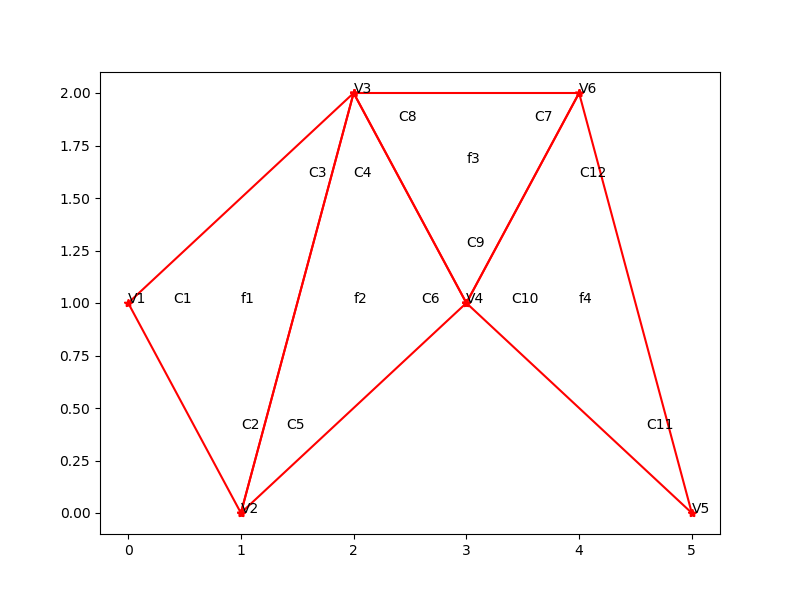
\includegraphics[width=1.0\textwidth]{example1.png}
 	\label{fig:example1} 
 	\caption[caption]{Exemplo 1 - Gráfico da página 80}
 \end{figure}
 
 
 \begin{figure}[ht]
	\centering
	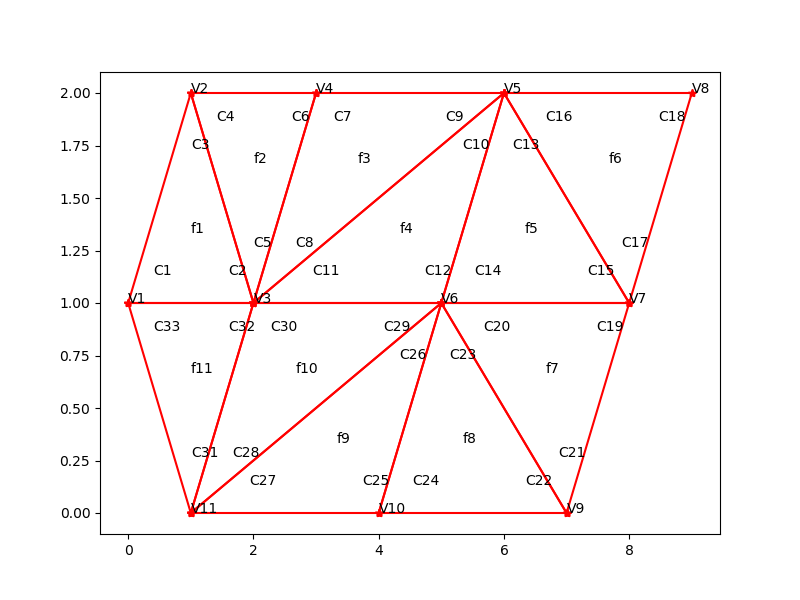
\includegraphics[width=1.0\textwidth]{example2.png}
	\label{fig:example2} 
	\caption[caption]{Exemplo 2 -Gráfico da página 21}
\end{figure}
 
 
 
 A implementação da \textit{corner table} recebe as duas estruturas lidas, uma com a posição física dos vértices, e outra com a definição das faces. Embora essa segunda seja modificada para receber apenas a lista de vértices, isso é necessário pois o \textit{VTK} traz na frente de cada lista de vértices das faces o número de vértices utilizados em cada face, e esse primeiro elemento não é necessário.
 
 O cômputo da \textit{corner table} é feito em 3 passadas. A primeira cria todos os \textit{corners}, define quais são os vértices pertencentes, e suas faces. Na segunda passada são calculados para cada \textit{corner} o próximo e \textit{corner} anterior. E na terceira passadas são encontrados as informações restantes da tabela, \textit{corners} oposto, esquerdo e direito. Durante a primeira passada também é criada uma lista indexada pelos vértices que retorna quais \textit{corners} esse vértice está relacionado.
 
 Abaixo temos as \textit{corners table} para os exemplos 1 e 2, figuras \ref{fig:example1} e \ref{fig:example2}.
 
 \begin{tabular}{rrrrrrrr}
 	\hline
 	Corner &   Vertice &   Face &   Next &   Previous &   Opposite &   Left &   Right \\
 	\hline
 	-1 &        -1 &     -1 &     -1 &         -1 &         -1 &     -1 &      -1 \\
 	1 &         1 &      1 &      2 &          3 &          6 &     -1 &      -1 \\
 	2 &         2 &      1 &      3 &          1 &         -1 &     -1 &       6 \\
 	3 &         3 &      1 &      1 &          2 &         -1 &      6 &      -1 \\
 	4 &         3 &      2 &      5 &          6 &         -1 &      7 &       1 \\
 	5 &         2 &      2 &      6 &          4 &          7 &      1 &      -1 \\
 	6 &         4 &      2 &      4 &          5 &          1 &     -1 &       7 \\
 	7 &         6 &      3 &      8 &          9 &          5 &     11 &      -1 \\
 	8 &         3 &      3 &      9 &          7 &         11 &     -1 &       5 \\
 	9 &         4 &      3 &      7 &          8 &         -1 &      5 &      11 \\
 	10 &         4 &      4 &     11 &         12 &         -1 &      8 &      -1 \\
 	11 &         5 &      4 &     12 &         10 &          8 &     -1 &      -1 \\
 	12 &         6 &      4 &     10 &         11 &         -1 &     -1 &       8 \\
 	\hline
 \end{tabular}



\begin{tabular}{rrrrrrrr}
	\hline
	Corner &   Vertice &   Face &   Next &   Previous &   Opposite &   Left &   Right \\
	\hline
	-1 &        -1 &     -1 &     -1 &         -1 &         -1 &     -1 &      -1 \\
	1 &         1 &      1 &      2 &          3 &          6 &     -1 &      31 \\
	2 &         3 &      1 &      3 &          1 &         -1 &     31 &       6 \\
	3 &         2 &      1 &      1 &          2 &         31 &      6 &      -1 \\
	4 &         2 &      2 &      5 &          6 &          9 &     -1 &       1 \\
	5 &         3 &      2 &      6 &          4 &         -1 &      1 &       9 \\
	6 &         4 &      2 &      4 &          5 &          1 &      9 &      -1 \\
	7 &         4 &      3 &      8 &          9 &         12 &     -1 &       4 \\
	8 &         3 &      3 &      9 &          7 &         -1 &      4 &      12 \\
	9 &         5 &      3 &      7 &          8 &          4 &     12 &      -1 \\
	10 &         5 &      4 &     11 &         12 &         28 &     15 &       7 \\
	11 &         3 &      4 &     12 &         10 &         15 &      7 &      28 \\
	12 &         6 &      4 &     10 &         11 &          7 &     28 &      15 \\
	13 &         5 &      5 &     14 &         15 &         21 &     18 &      11 \\
	14 &         6 &      5 &     15 &         13 &         18 &     11 &      21 \\
	15 &         7 &      5 &     13 &         14 &         11 &     21 &      18 \\
	16 &         5 &      6 &     17 &         18 &         -1 &     -1 &      14 \\
	17 &         7 &      6 &     18 &         16 &         -1 &     14 &      -1 \\
	18 &         8 &      6 &     16 &         17 &         14 &     -1 &      -1 \\
	19 &         7 &      7 &     20 &         21 &         24 &     -1 &      13 \\
	20 &         6 &      7 &     21 &         19 &         -1 &     13 &      24 \\
	21 &         9 &      7 &     19 &         20 &         13 &     24 &      -1 \\
	22 &         9 &      8 &     23 &         24 &         27 &     -1 &      19 \\
	23 &         6 &      8 &     24 &         22 &         -1 &     19 &      27 \\
	24 &        10 &      8 &     22 &         23 &         19 &     27 &      -1 \\
	25 &        10 &      9 &     26 &         27 &         30 &     -1 &      22 \\
	26 &         6 &      9 &     27 &         25 &         -1 &     22 &      30 \\
	27 &        11 &      9 &     25 &         26 &         22 &     30 &      -1 \\
	28 &        11 &     10 &     29 &         30 &         10 &     33 &      25 \\
	29 &         6 &     10 &     30 &         28 &         33 &     25 &      10 \\
	30 &         3 &     10 &     28 &         29 &         25 &     10 &      33 \\
	31 &        11 &     11 &     32 &         33 &          3 &     -1 &      29 \\
	32 &         3 &     11 &     33 &         31 &         -1 &     29 &       3 \\
	33 &         1 &     11 &     31 &         32 &         29 &      3 &      -1 \\
	\hline
\end{tabular}\\~\\

 
 
 A primeira linha é deixada com valores -1 para a numeração dos \textit{corners} começar em 1. E o valores -1 na tabela indica vazio.
 
 Os comandos para gerar cada tabela foram:
 
 \begin{itemize}
\item Exemplo 1:
\begin{verbatim}
import corner_table as cnt
ex1 = cnt.read_vtk("example1.vtk")
ex1_corner = cnt.compute_corner_table(ex1[0], ex1[1][:, [1,2,3]])
\end{verbatim}

\item Exemplo 2:
\begin{verbatim}
import corner_table as cnt
ex2 = cnt.read_vtk("example2.vtk")
ex2_corner = cnt.compute_corner_table(ex2[0], ex2[1][:, [1,2,3]])
\end{verbatim}
 \end{itemize}
 
 
 Além da criação da estrutura também foi pedido para implementar algumas operações utilizando a estrutura.
 No código disponibilizado estão implementados todos os métodos descritos nos \textit{slides}, fecho, estrela, link, e 1-anel.

 Todas essas operações têm como parâmetros a \textit{corner table}, a lista dos \textit{corners} em cada vértices, e os pontos de consulta separados por tipo, vértice, aresta e face.
 
Exemplo da utilização dos métodos nos grafos analisados anteriormente.


\begin{itemize}
	\item Exemplo 1:
	\begin{itemize}
		\item Fecho do vértice 4:
		
		Execução do código e resposta:
		\begin{verbatim}
		cnt.closure(ex1_corner[1], ex1_corner[0], vt=[4], ed=[], fc=[])
		{'vertices': {4}, 'edges': set(), 'faces': set()}
		\end{verbatim}
		
		\item Estrela da aresta (3,4):
		
		Execução do código e resposta:
		\begin{verbatim}
		cnt.star(ex1_corner[1], ex1_corner[0], vt=[], ed=[(3,4)], fc=[])
		{
		'vertices': {3, 4}, 
		'edges': {
		frozenset({2, 4}), frozenset({3, 6}), 
		frozenset({3, 4}), frozenset({2, 3}), 
		frozenset({4, 6}), frozenset({1, 3}), 
		frozenset({4, 5})
		}, 
		'faces': {1, 2, 3, 4}
		}
		\end{verbatim}
		
		\item \textit{Link} da aresta (3,4):
		
		Execução do código e resposta:
		\begin{verbatim}
		cnt.link(ex1_corner[1], ex1_corner[0], vt=[], ed=[(3,4)], fc=[])
		{
		'vertices': {1, 2, 5, 6}, 
		'edges': {frozenset({1, 2}), frozenset({5, 6})}, 
		'faces': set()
		}
		\end{verbatim}
		
	\end{itemize}
	
	
	
	\item Exemplo 2:
	\begin{itemize}
		\item Fecho da face 3 (f3) e da aresta entre os vértices 6 e 9:
		 \begin{figure}[ht]
			\centering
			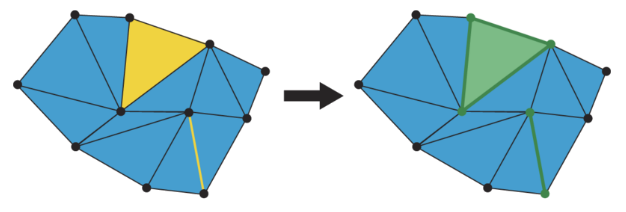
\includegraphics[width=1.0\textwidth]{fecho_ex2.png}
			\label{fig:fecho_ex2}
			\caption[caption]{Fecho do exemplo 2 para f3 e (V6-V9)}
		\end{figure}
		
		Execução do código e resposta:
		\begin{verbatim}
cnt.closure(ex2_corner[1], ex2_corner[0], vt=[], ed=[(6,9)], fc=[3])
{ 
	'vertices': {3, 4, 5, 6, 9}, 
	'edges': {
		frozenset({3, 4}), frozenset({3, 5}), 
		frozenset({9, 6}), frozenset({4, 5})
	}, 
	'faces': {3}
}
		\end{verbatim}
		
		\item Estrela do vértice 3 (V3):
		\begin{figure}[ht]
			\centering
			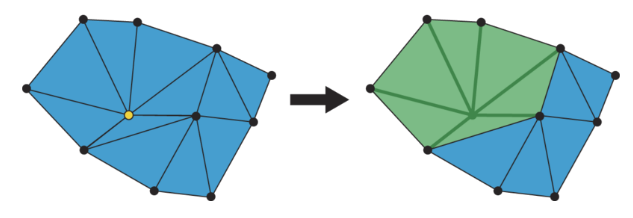
\includegraphics[width=1.0\textwidth]{estrela_ex2.png}
			\label{fig:estrela_ex2}
			\caption[caption]{Estrela do exemplo 2 para V3}
		\end{figure}
		
		Execução do código e resposta:
		\begin{verbatim}
		cnt.star(ex2_corner[1], ex2_corner[0], vt=[3], ed=[], fc=[])
		{
		'vertices': {3}, 
		'edges': {
		frozenset({3, 6}), frozenset({3, 5}), 
		frozenset({3, 4}), frozenset({2, 3}), 
		frozenset({11, 3}), frozenset({1, 3})
		}, 
		'faces': {1, 2, 3, 4, 10, 11}
		}
		\end{verbatim}
		
		\item \textit{Link} do vértice 3 (V3):
		\begin{figure}[ht]
			\centering
			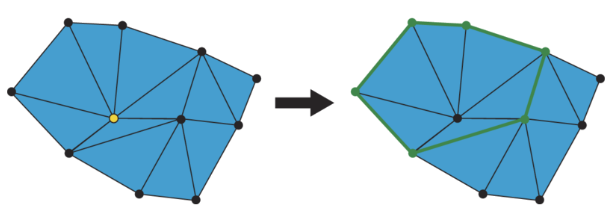
\includegraphics[width=1.0\textwidth]{link_ex2.png}
			\label{fig:link_ex2}
			\caption[caption]{\textit{Link} do exemplo 2 para V3}
		\end{figure}
		
		Execução do código e resposta:
		\begin{verbatim}
		cnt.link(ex2_corner[1], ex2_corner[0], vt=[3], ed=[], fc=[])
		{
		'vertices': {1, 2, 4, 5, 6, 11}, 
		'edges': {
		frozenset({2, 4}), frozenset({1, 11}), 
		frozenset({1, 2}), frozenset({5, 6}), 
		frozenset({4, 5}), frozenset({11, 6})
		}, 
		'faces': set()
		}
		\end{verbatim}
		
	\end{itemize}
\end{itemize}


Com os exemplos acima verificou-se que a implementação está correta, e para avaliar o desempenho foi disponibilizada um arquivo \textit{VTK} com 836 vértices e 1696 faces. Mesmo utilizando um malha dessa dimensão o carregamento e construção da \textit{corner table} foi quase instantâneo. E a complexidade das operações também é muito baixa utilizando a \textit{corner table}.
 Abaixo é exibida a utilização da implementação para o arquivo \textit{socket.vtk}.

\begin{verbatim}
>>> socket = cnt.read_vtk('socket.vtk')
>>> socket_corner = cnt.compute_corner_table(socket[0], socket[1][:, [1,2,3]])

>>> cnt.closure(socket_corner[1], socket_corner[0], vt=[40], ed=[], fc=[])                 
{'vertices': {40}, 'edges': set(), 'faces': set()}
>>> cnt.closure(socket_corner[1], socket_corner[0], vt=[], ed=[(31,32)], fc=[])  

{'vertices': {32, 31}, 'edges': {frozenset({32, 31})}, 'faces': set()}
>>> cnt.closure(socket_corner[1], socket_corner[0], vt=[], ed=[(40,41)], fc=[])       

{'vertices': {40, 41}, 'edges': {frozenset({40, 41})}, 'faces': set()}
>>> cnt.closure(socket_corner[1], socket_corner[0], vt=[], ed=[(400,401)], fc=[])

{'vertices': {400, 401}, 'edges': {frozenset({400, 401})}, 'faces': set()}
>>> cnt.closure(socket_corner[1], socket_corner[0], vt=[], ed=[], fc=[100])      
{'vertices': {33, 34, 428}, 
'edges': {frozenset({34, 428}), frozenset({33, 34}), 
frozenset({33, 428})}, 
'faces': {100}}
>>> 
>>> 
>>> cnt.closure(socket_corner[1], socket_corner[0], vt=[], ed=[], fc=[10,20,30])
{'vertices': {397, 398, 400, 401, 406, 407, 409, 410, 411}, 
'edges': {frozenset({400, 398}), frozenset({406, 407}), 
frozenset({411, 397}), frozenset({409, 406}), 
frozenset({401, 398}), frozenset({410, 411}),
 frozenset({410, 397}), frozenset({409, 407}), 
 frozenset({400, 401})}, 
 'faces': {10, 20, 30}}
>>> 

>>> 
>>> cnt.star(socket_corner[1], socket_corner[0], vt=[101], ed=[], fc=[])               
{'vertices': {101}, 
'edges': {frozenset({101, 431}), frozenset({101, 102}), 
frozenset({432, 101}), frozenset({593, 101}), 
frozenset({592, 101}), frozenset({100, 101})}, '
faces': {165, 166, 169, 751, 752, 760}}
>>> 
>>> 
>>> 
>>> 
>>> cnt.star(socket_corner[1], socket_corner[0], vt=[101,300], ed=[], fc=[])
{'vertices': {300, 101}, 
'edges': {frozenset({810, 300}), frozenset({300, 367}), 
frozenset({101, 431}), frozenset({101, 102}), 
frozenset({300, 311}), frozenset({300, 301}), 
frozenset({592, 101}), frozenset({300, 366}), 
frozenset({593, 101}), frozenset({432, 101}), 
frozenset({300, 647}), frozenset({100, 101})}, 
'faces': {833, 834, 1603, 1604, 1605, 1606, 165, 166, 169, 751, 752, 760}}
>>> 
>>> 
>>> 
>>> 
>>> 
>>> cnt.link(socket_corner[1], socket_corner[0], vt=[101,200], ed=[], fc=[])            
{'vertices': {544, 547, 100, 102, 199, 201, 431, 592, 593, 432, 761, 379}, 
'edges': {frozenset({102, 431}), frozenset({593, 102}), 
frozenset({761, 379}), frozenset({544, 199}), 
frozenset({379, 199}), frozenset({432, 100}),
 frozenset({761, 201}), frozenset({201, 547}), 
 frozenset({432, 431}), frozenset({592, 100}), 
 frozenset({544, 547}), frozenset({592, 593})}, 
 'faces': set()}

\end{verbatim}




\end{document}
